% !TEX root = DesignDocument.tex


\chapter{System  and Unit Testing}

This section will discuss the testing methods that the design team used during the development of the Virtual Museum.  Due to the nature of the project, unit tests and other testing methods weren't exactly applicable to the project.  Because of this, the design team had to utilize other testing methods, which will be covered further in this section.

\section{Overview}
Throughout the development of this project, there was much testing to make sure the objects and actors worked together in the Engine.  The design team looked for graphical errors such as tearing of textures, objects clipping through walls, etc.  Other things that were tested as the project grew were key presses doing the expected action, and above all else the design team made sure the Oculus performed as highly as possible after each sprint was completed.  This was to ensure that the user would feel immersed in the gallery and that the features would not detract from that.  

As for unit testing, there was no way to generate unit tests in the Unreal Engine so testing was more focused on user experience and mitigating simulation sickness.  However, the on-rails movement system needed to be thoroughly tested to make sure that the "next-painting" button would in fact take you to the next painting and not somewhere else entirely.  This resulted in the tedious process of navigating to and from each painting in the gallery.

The other features were slightly more easy to test.  Free-movement was tested every time the design team needed to enter the gallery to make sure the newest feature was behaving correctly.  Text-descriptions were all individually tested to make sure their animations didn't cause the object to clip through neighboring walls and also to make sure the text was legible at a reasonable distance.  The alternate environment was tested simply by testing the button that transports the user to it.  The environment itself was an Unreal Engine object with textures and scenery applied to it, so testing was focused on making it feel immersive to the user.


\section{Test Setup and Execution}
In many other projects, testing is done by having a test with an expected output, and if the test produces something else, then you know something is wrong.  In the Virtual Museum, that method of testing does not cover what is needed for the quality of the project.  Of course there are features that can be tested in this way and these are:
	\begin{description}
	\item[On-rails movement] \hfill \\
		This feature had the most involved testing process because at every painting both: forward and 				backward transitions had to be tested.  With around 50 paintings, that resulted in around 100 test 		cases that had to be done. 
	\item [Free-movement] \hfill \\
		As stated earlier in this section, this was the first feature to be implemented and was tested 				every time either Alex or Mack needed to enter the gallery.  In addition to that amount of 					testing, the design team also made sure to walk along every wall to make sure there was no 					clipping possible.
	\item [Text-description animations] \hfill \\
		Since each test description used the same blueprint to handle the animation, the testing was focused around making sure the animation didnt cause the text box to clip through walls.  In order to do this, the design team had to go to each text description and make sure it animated to the desired position.  This proved difficult for the descriptions located in the corners because they liked to clip through the adjacent wall.
	\item[Alternate environment transport button] \hfill \\
		This was probably the easiest thing to test, because it was a button that had one function: toggle the environment variable on or off.  When it is pressed the first time, the variable is set to true and the user transported to the alternate environment.  When it is pressed the second time, it takes the user back to the gallery, and so on...
	\end{description}
	
	\end{enumerate}


\section{Risk Analysis}
There were a number of possible risks that were associated with this project.  The main risk being simulation sickness, the motion-sickness that afflicts a lot of virtual reality users.  Because simulation sickness is such a huge factor in user experience, the design team spent most of sprint 3 testing different movement speeds and other factors that cause the sickness.
Other risks that were associated with the project include:
	\begin{enumerate}
	\item Oculus Rift not conducive to people with glasses
	\item The actual headset could get very gross with many people using the same one
	\item The text in the text-descriptions might be too advanced for younger users
	\item Others that the design team couldn't think of
	\end{enumerate}
As you can tell, some of these risks are outside the scope of the project, so the mitigation will have to be done by the Dahl if they decide to continue this project. 
\subsection{Risk Mitigation}
The main method used for mitigating simulation sickness was to survey as many users as possible to find what worked and what didn't.  Since the majority of simulation sickness comes from movement in the virtual environment, the survey from sprint 3 asked users to rate how sick they felt after moving around the gallery with both movement methods.  The results are a little hard to read at first glance, to clarify, the motion sickness index represents how easily that user gets motion sick.  After that, the results show that in general, on-rails movement caused less sickness than free-movement which was inline with the team's predictions.  This also follows the Oculus Rift development model as well; the Oculus documentation suggests limiting user-controlled movement due to the fact that it causes more sickness.  This was the reasoning behind the on-rails movement, however the design team wanted to include free-movement and let the Dahl decide which movement they liked more.
\begin{figure}
\centering
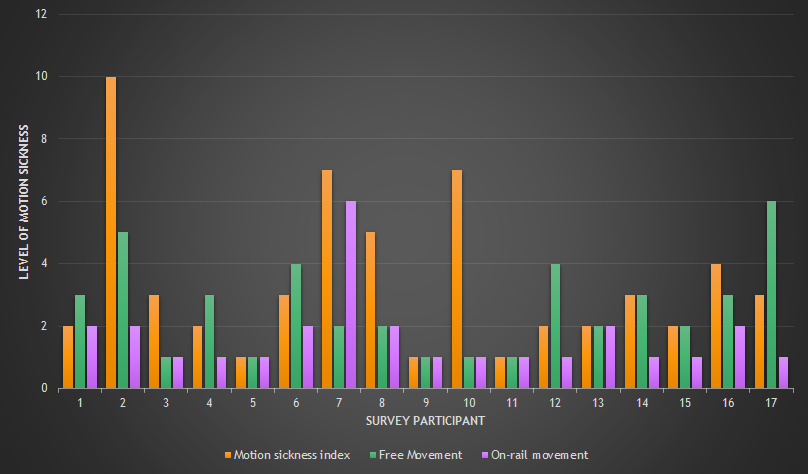
\includegraphics[scale=0.5]{Diagrams/surveyresults.png}
\caption{Results from the survey}
\end{figure}
\section{Successes, Issues and Problems}
\subsection{Successes}
Overall, the movement styles fit the project very well.  The somewhat slow movement speed is what you would expect when visiting an art museum in real life, and this provides an additional sense of immersion for the user.  In addition to the movement speed, the on-rails movement system works very well by gradually sliding the user from painting to painting at a very reasonable speed.  It also works very well with the text-description animations, when the user goes to the next painting the current text-description will shrink back down so the user doesn't slide through it. 

\subsection{Issues and Problems}
Although it was stated as a success, the movement speed was at the center of much debate with the design team and the testing users.  The users wanted faster movement, but the design team thought that the slower speed was more reasonable for the project.  
One other problem that came up was during the alternate environment sprint.  This is a minor issue because it doesn't affect the gallery in any way, it only affects user immersion and even then, most users didn't seem to notice.  The issue is that the scenery in the alternate environment: trees, grass, shrubs... are not authentic to the Black Hills.  This was mentioned earlier in the document but should be restated here, that there were no available Unreal Engine assets that accurately represented the flora of the Black Hills, such as the Ponderosa Pine tree.  Although this is a minor issue, if the Dahl continues this project, this problem should be addressed by either finding the assets, or creating them in-house with some sort of graphics program.

\subsection{Changes to the Backlog}
Because there were only minor issues that came up, there were no changes to the backlog in any of the sprints.

